\section{Fahrcontroller}
\begin{frame}
\frametitle{Fahrcontroller}
\framesubtitle{Kalibrierung}

\begin{columns}
	\begin{column}{0.42 \textwidth}
		\begin{itemize}
			\item Berechnung automatisiert
			\item Bedienung vereinfacht
		\end{itemize}
	\end{column}
	\begin{column}{0.58 \textwidth}
		\vspace{-2.8em}
		\begin{figure}[h]
			\centering
			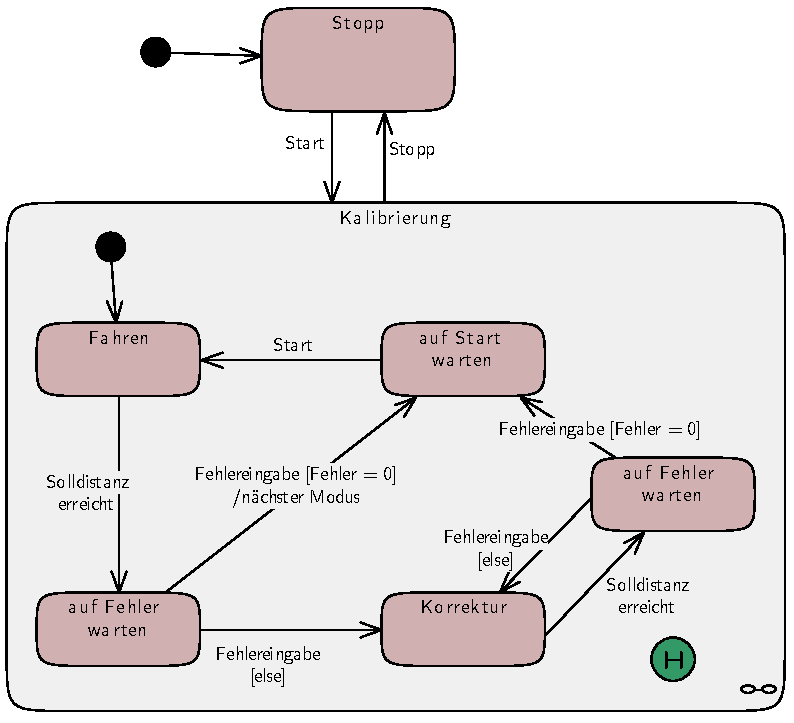
\includegraphics[width = 1 \textwidth]{../images/DC/calSMPres}
		\end{figure}
	\end{column}
\end{columns}

\end{frame}

\begin{frame}
\frametitle{Fahrcontroller}
\framesubtitle{Positionsregelung}

\begin{columns}
	\begin{column}{0.53 \textwidth}
		\begin{itemize}
			\item Regelung statt Steuerung
			\item Punkte müssen nicht genau angefahren werden
			\item Höhere Durchschnittsgeschwindigkeit
		\end{itemize}
	\end{column}
	\begin{column}{0.47 \textwidth}
		\vspace{-4em}
		\begin{figure}[h]
			\centering
			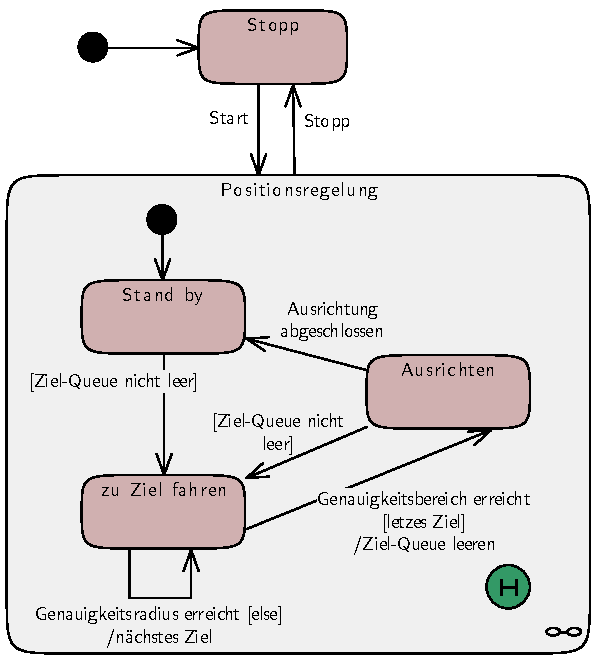
\includegraphics[width = 1.02 \textwidth]{../images/DC/PosControlPres.pdf}
		\end{figure}
	\end{column}
\end{columns}

\end{frame}

\begin{frame}
\frametitle{Fahrcontroller}
\framesubtitle{Demo}

\begin{columns}
	\begin{column}{0.4 \textwidth}
		\begin{itemize}
			\item Richtung wählbar
			\item Genauigkeit einstellbar
			\item verschiedene Modi
		\end{itemize}
	\end{column}
	\begin{column}{0.6 \textwidth}
		\begin{tikzpicture}[scale = 1.15, transform shape]	
			\draw [fill = hsrBlue] (0, 0) circle (2pt) node[above, color=black]{1,7};
			\draw [-, line width = 0.2mm, hsrBlue] (0, 0) -- (1, 0);
			\draw [fill = hsrBlue] (1, 0) circle (2pt) node[above, color=black]{2};
			\draw [-, line width = 0.2mm, hsrBlue] (1, 0) -- (2, 1);
			\draw [fill = hsrBlue] (2, 1) circle (2pt) node[above, color=black]{3};
			\draw [-, line width = 0.2mm, hsrBlue] (2, 1) -- (4, 1);
			\draw [fill = hsrBlue] (4, 1) circle (2pt) node[above, color=black]{4};
			\draw [-, line width = 0.2mm, hsrBlue] (4, 1) -- (5, 0);
			\draw [fill = hsrBlue] (5, 0) circle (2pt) node[above, color=black]{5};
			\draw [-, line width = 0.2mm, hsrBlue] (5, 0) -- (6, 0);
			\draw [fill = hsrBlue] (6, 0) circle (2pt) node[above, color=black]{6};
			\draw [-, line width = 0.2mm, hsrBlue] (5, 0) -- (3, 0);
			\draw [-, line width = 0.2mm, hsrBlue] (3, 0) -- (1, 0);
		\end{tikzpicture}
	\end{column}
\end{columns}

\end{frame}
